\chapter{随机变量及其分布}\label{ch:02}
\chaptermap{随机变量\\分布函数}{离散与连续\\常见分布}{函数分布\\逆像与导数}{独立和\\卷积与母函数}
\begin{examtip}
\textbf{考研核心：}分布函数的跳跃、密度归一化、常用分布及函数的分布。
\textbf{竞赛视角：}概率积分变换、无记忆性和生成函数。
\textbf{测度关联：}随机变量是可测函数；分布既可能有原子，也可能有连续部分，甚至有奇异连续部分。
\end{examtip}
\section{分布函数与混合型分布}\label{sec:21}
\src{茆诗松, §2.1；李东风, §2.1、§2.4}
\begin{definition}{随机变量与分布函数}
实函数$X:\Omega\to\R$若对每个$x\in\R$都有$\{\omega:X(\omega)\le x\}\in\Fcal$，称为随机变量。
$F_X(x)=\Pp(X\le x)$非减、右连续，且两端极限分别为0和1。
$\Pp(a<X\le b)=F_X(b)-F_X(a)$，$\Pp(X=x)=F_X(x)-F_X(x-)$。
若存在非负可积函数$f$使每个$x$都有$F(x)=\int_{-\infty}^xf(t)\dd t$，称$X$为连续型随机变量，$f$为密度，且$\int_\R f=1$；测度语言称此分布绝对连续。
密度按Lebesgue几乎处处相等识别。仅有CDF连续只保证没有原子，未必有密度，反例见例\ref{ex:10-6}。
\end{definition}
\begin{proof}
非减性来自事件包含。若$x_n\downarrow x$，则$\{X\le x_n\}\downarrow\{X\le x\}$，概率连续性给右连续；两端极限同理。
区间差公式来自不交分解，单点质量来自$\{X<x\}$的递增逼近。
\end{proof}
\begin{method}{跳跃与光滑部分分开算}
适用：给定分布函数、截断或门限输出。先检查端点、单调、右连续；跳跃量给原子质量，开区间导数给连续密度。
不能对分布函数求导后就丢弃全部跳跃。
\end{method}
\worked{正部截断}{基础例题}{\star\star}{2-1}
{$X\sim U(-1,1)$，$Y=\max(X,0)$，求$Y$分布。}
{把负半轴压缩产生的原子单列。}
{方法一：$y<0$时$F_Y(y)=0$；$0\le y<1$时$\{Y\le y\}=\{X\le y\}$，故$F_Y(y)=\frac{y+1}{2}$；$y\ge1$时为1。
方法二：$X\le0$的概率$\frac{1}{2}$全部落在0，其余在$(0,1)$保留密度$\frac{1}{2}$。
所以分布为$\frac12\delta_0+\frac12U(0,1)$。}
{CDF自动保留原子；分块映射法更易解释质量来源。}
{$Y$没有一个相对于Lebesgue测度的普通密度能表示全部概率。}
\worked{从CDF读端点}{考研风格}{\star}{2-2}
{设$F(x)=0$（$x<0$），$F(x)=\frac{1}{3}+\frac{x}{3}$（$0\le x<2$），$F(x)=1$（$x\ge2$）。求$\Pp(X=0)$及$\Pp(0<X\le1)$。}
{分别看跳跃与区间增量。}
{$F(0)-F(0-)=\frac{1}{3}$；$F(1)-F(0)=\frac{2}{3}-\frac{1}{3}=\frac{1}{3}$。
在$(0,2)$密度为$\frac{1}{3}$，积分为$\frac{2}{3}$，加0处原子后总质量为1。
在2处左极限为1，因此没有额外原子。}
{端点是否有质量决定开闭区间能否交换。}
{本例$\Pp(0\le X\le1)=\frac{2}{3}$，与题中事件不同。}
\worked{CDF的广义逆抽样}{竞赛风格}{\star\star\star}{2-3}
{$U\sim U(0,1)$，$Q(u)=\inf\{x:F(x)\ge u\}$。证明$Q(U)$分布函数为$F$。}
{把逆像事件化为均匀变量的不等式。}
{由非减和右连续性，对$0<u<1$有$Q(u)\le x$当且仅当$u\le F(x)$。
正向可用右连续性保证下确界处达到该水平；逆向因$x$本身已在上水平集中而成立。
所以$\Pp(Q(U)\le x)=\Pp(U\le F(x))=F(x)$。}
{广义逆对离散、连续和混合分布统一有效。}
{有跳跃时普通反函数不存在；不能随意写$F^{-1}$而不说明广义逆。}

\section{离散分布族}\label{sec:22}
\src{茆诗松, §2.4；李东风, §2.2}
\begin{definition}{常用离散模型}
Bernoulli$(p)$在0、1的概率分别为$1-p,p$；$\Bin(n,p)$质量为$\binom nkp^k(1-p)^{n-k}$，$k=0,\ldots,n$，其中$0\le p\le1$、$n$为非负整数，端点按退化分布理解。
$\Pois(\lambda)$质量为$\frac{e^{-\lambda}\lambda^k}{k!}$（$k=0,1,\ldots$），通常取$\lambda>0$；允许$\lambda=0$时约定为0点的退化分布。
几何分布质量为$p(1-p)^{k-1}$（$k=1,2,\ldots$），$0<p\le1$，$p=1$时恒为1。
超几何参数$N\ge1$、$0\le M,n\le N$均为整数，质量为$\frac{\binom Mk\binom{N-M}{n-k}}{\binom Nn}$，支持为
$\max(0,n-N+M)\le k\le\min(n,M)$的整数。以上质量在各自支持外均为0。
\end{definition}
\begin{method}{用抽样机制识别分布}
适用：重复成功数、稀有计数、首次成功与不放回抽样。先写取值，再匹配质量函数；求概率时先检查支持边界。
二项需要独立同成功率；超几何允许抽次间相关。
\end{method}
\worked{二项与超几何的比较}{基础例题}{\star\star}{2-4}
{10件中4件次品，抽3件，求恰有1次品概率，分别考虑放回和不放回。}
{比较独立计数与组合计数。}
{放回：方法一按二项得$\binom31(0.4)(0.6)^2=0.432$；方法二指定次品所在的三个位置，每个概率$0.4(0.6)^2$，相加相同。
不放回：$\frac{\binom41\binom62}{\binom{10}3}=\frac{1}{2}$。
两种机制的每次边缘次品率都为$0.4$，但联合结构不同。}
{独立性是区分两种计数分布的关键。}
{边缘成功率不变不意味着各次独立。}
\worked{Poisson的条件计数}{考研风格}{\star\star}{2-5}
{独立$X\sim\Pois(a),Y\sim\Pois(b)$，求$X\given X+Y=n$的分布。}
{写联合质量并归一化。}
{对$0\le k\le n$，分子为$\frac{e^{-(a+b)}a^kb^{n-k}}{k!(n-k)!}$。
分母由二项展开为$\frac{e^{-(a+b)}(a+b)^n}{n!}$，故条件质量
$\binom nk\{\frac{a}{a+b}\}^k\{\frac{b}{a+b}\}^{n-k}$。
所以是$\Bin(n,\frac{a}{a+b})$，假设$a+b>0$。}
{独立Poisson之和与条件二项是一对互补结构。}
{当$n\ge1$且$a,b>0$时，给定$X+Y=n$后$X,Y$不独立；当$n=0$或某一率为0时，条件分布退化，$X,Y$仍可独立。}
\worked{几何分布的奇偶性}{考研风格}{\star\star}{2-6}
{$N$为成功率$p\in(0,1)$的几何变量，求$\Pp(N\text{为奇数})$。}
{按奇数尾求几何级数。}
{令$q=1-p$，则$\sum_{j\ge0}pq^{2j}=\frac{p}{1-q^2}=\frac{1}{2-p}$。
也可设所求为$r$，首轮成功给$p$；首轮失败后总次数奇数要求余下次数偶数，故$r=p+q(1-r)$，解得同式。}
{级数法直接；首轮分解可迁移到更复杂的周期状态。}
{不能因奇偶各占一半整数就判断概率各半。}

\section{连续分布族与分位数}\label{sec:23}
\src{茆诗松, §2.5；李东风, §2.3}
\begin{definition}{常用连续模型}
$U(a,b)$要求$a<b$，密度为$(b-a)^{-1}\ind_{(a,b)}(x)$；$\Exp(\lambda)$要求$\lambda>0$，密度为$\lambda e^{-\lambda x}\ind_{(0,\infty)}(x)$。
$\Ga(a,\lambda)$要求$a,\lambda>0$，密度为$\frac{\lambda^ax^{a-1}e^{-\lambda x}}{\Gamma(a)}$（$x>0$）；$\Normal(\mu,\sigma^2)$要求$\mu\in\R,\sigma>0$，在全实轴的密度为$\frac{e^{-\frac{(x-\mu)^2}{2\sigma^2}}}{\sqrt{2\pi}\sigma}$。
$\Beta(a,b)$要求$a,b>0$，密度为$\frac{x^{a-1}(1-x)^{b-1}}{B(a,b)}$（$0<x<1$）。除正态外，上述密度在指定支持外均为0。
其中$\lambda$统一为率，$\Gamma(a)=\int_0^\infty t^{a-1}e^{-t}\dd t$，$B(a,b)=\int_0^1t^{a-1}(1-t)^{b-1}\dd t$。
对$0<u<1$，下侧分位数定义为$q_u=\inf\{x:F(x)\ge u\}$。中位数$m$满足$\Pp(X\le m)\ge\frac{1}{2}$且$\Pp(X\ge m)\ge\frac{1}{2}$；CDF连续时可用$F(m)=\frac{1}{2}$，离散情形不可强求这个等式。
\end{definition}
\begin{theorem}{指数无记忆与正态标准化}
若$X\sim\Exp(\lambda)$，则对所有$s,t\ge0$，有$\Pp(X>s+t\given X>s)=e^{-\lambda t}$。
若$X\sim\Normal(\mu,\sigma^2)$，则$\frac{X-\mu}{\sigma}\sim\Normal(0,1)$。
\end{theorem}
\begin{proof}
前式用尾概率比$\frac{e^{-\lambda(s+t)}}{e^{-\lambda s}}$。
后式令$x=\mu+\sigma z$，密度乘雅可比$\sigma$，化为标准正态密度。
\end{proof}
\begin{method}{标准化与尾部方向}
适用：正态区间、指数寿命、分位数。先把事件化成标准变量，再用$\Phi$或尾指数计算。
使用$z_u$统一下侧分位数，右尾水平$\alpha$对应$z_{1-\alpha}$。
\end{method}
\worked{指数的分位数}{基础例题}{\star}{2-7}
{$X\sim\Exp(2)$，求中位数和$\Pp(X>2\given X>1)$。}
{以CDF和尾概率两条路线求中位数。}
{方法一：$1-e^{-2m}=\frac{1}{2}$得$m=\frac{\log2}{2}$；条件概率为$\frac{e^{-4}}{e^{-2}}=e^{-2}$。
方法二：中位数将尾概率也分成$\frac{1}{2}$，直接解$e^{-2m}=\frac{1}{2}$；无记忆性使条件剩余寿命超过1的概率为$e^{-2}$。}
{两法分别强调累计概率和剩余寿命。}
{率为2时均值为$\frac{1}{2}$，不能把率当均值。}
\worked{正态反求参数}{考研风格}{\star\star}{2-8}
{$X\sim\Normal(\mu,\sigma^2)$，已知$\Pp(X\le2)=\frac{1}{2}$、$\Pp(X\le5)=\Phi(1.5)$，求参数。}
{正态对称中心是唯一中位数。}
{由严格递增性，$\frac{2-\mu}{\sigma}=0$，得$\mu=2$。
再由$\frac{5-2}{\sigma}=1.5$，得$\sigma=2$，方差为4。
检查：5比均值高$1.5$个标准差，与给定分布函数值相符。}
{反求分布参数就是把概率等式转为标准分位数方程。}
{标准差与方差不能在标准化分母中互换。}
\worked{连续无记忆性的刻画}{竞赛风格}{\star\star\star}{2-9}
{非负有限随机变量尾函数$G(t)>0$满足$G(s+t)=G(s)G(t)$且$G(0)=1$，证明其为指数分布。}
{对尾函数取负对数并利用单调性。}
{令$h(t)=-\log G(t)$，则$h(s+t)=h(s)+h(t)$且非减。
整数与有理数上$h(q)=qh(1)$；任意实数$t\ge0$用上下有理数逼近，单调性夹得$h(t)=\lambda t$。
有限性给$G(t)\downarrow0$，故$\lambda>0$，于是$G(t)=e^{-\lambda t}$。}
{概率的单调性排除了Cauchy方程的病态解。}
{若允许$X=+\infty$，$\lambda=0$的退化尾函数也可能出现。}

\section{一元随机变量函数的分布}\label{sec:24}
\src{茆诗松, §2.6；Papoulis--Pillai, §5.2}
\begin{theorem}{多分支密度变换}
设$X$绝对连续，除一个$X$概率为0的集合外，其支持可分成有限或可数个不交区间。在每个区间上$g$为$C^1$、严格单调且$g'\ne0$，逆函数记为$x_j(y)$。则$Y=g(X)$有密度，几乎处处满足
\begin{equation}f_Y(y)=\sum_j f_X(x_j(y))\left|\dfrac{\dd x_j}{\dd y}\right|.\end{equation}
上式对有效分支求和，像集外密度为0。若另有常值区间，应先计算该区间映成的原子质量，再对其余满足条件的分支应用此式。
若导数为零的原像集合带有正概率，则还可能产生奇异部分，须回到CDF法，不能认定只有原子和上述密度。
\end{theorem}
\begin{proof}
先在单调区间把事件$Y\le y$转成$X$的区间，再对CDF求导；递减时导数的负号由绝对值吸收。
不同分支为不交来源，其概率相加得总密度。
\end{proof}
\begin{method}{先画像集，再列全部逆像}
适用：平方、绝对值、指数、倒数与分段变换。先求$Y$范围，再在每个单调分支求逆和导数，最后归一化。
CDF法适用面最广；密度法在分支少时计算更短。
\end{method}
\worked{平方变换的两法}{考研风格}{\star\star}{2-10}
{$X\sim U(-1,1)$，求$Y=X^2$的分布和密度。}
{平方是两对一变换。}
{方法一：$0\le y\le1$时$F_Y(y)=\Pp(-\sqrt y\le X\le\sqrt y)=\sqrt y$，故$f_Y(y)=\frac{1}{2\sqrt y}$。
方法二：两个逆像为$\pm\sqrt y$，每支贡献$\frac12\frac1{2\sqrt y}$，总和相同；范围外密度为0。
检查$\int_0^1(2\sqrt y)^{-1}\dd y=1$。}
{CDF法自然处理双分支；密度法要主动列全逆像。}
{$y=0$处密度无界并不表示原子，$\Pp(Y=0)=0$。}
\worked{正态指数变换}{考研风格}{\star\star}{2-11}
{$X\sim\Normal(\mu,\sigma^2)$，求$Y=e^X$密度。}
{映射严格递增，像集为正半轴。}
{$y>0$时$F_Y(y)=\Phi(\frac{\log y-\mu}{\sigma})$，求导得
\[f_Y(y)=\dfrac1{y\sigma\sqrt{2\pi}}\exp\!\left[-\dfrac{(\log y-\mu)^2}{2\sigma^2}\right].\]
$y\le0$时分布函数为0。这就是对数正态分布。}
{单调变换在CDF中直接反解不等式即可。}
{雅可比为$\frac{1}{y}$，漏掉后无法归一化。}
\worked{概率积分变换的边界}{测度论选学}{\star\star}{2-12}
{若$F$连续且严格递增，证明$F(X)\sim U(0,1)$；说明离散情形为何不成立。}
{使用反函数化事件。}
{对$0<u<1$，$\Pp(F(X)\le u)=\Pp(X\le F^{-1}(u))=u$。
若$X$是公平Bernoulli，$F(X)$只取$\frac{1}{2}$和1，各概率$\frac{1}{2}$，因而不服从连续均匀分布。
本节的严格递增条件可弱化为CDF连续，使用广义逆和零质量平坦区间可证。}
{从原变量映射到均匀变量需要连续性；从均匀变量经广义逆生成任意分布无需连续性。}
{两个方向的条件不对称。}

\section{卷积、和分布与生成函数}\label{sec:25}
\src{李东风, §3.4；Papoulis--Pillai, §6；生成函数统一表述}
\begin{theorem}{独立和的卷积与母函数}
独立连续$X,Y$的和有密度$f_{X+Y}(s)=\int_{\R}f_X(x)f_Y(s-x)\dd x$。
离散情形把积分改为对$x$求和。若矩母函数$M_X(t)=\E e^{tX}$与$M_Y(t)=\E e^{tY}$均在0的某个公共邻域内有限，则独立和满足$M_{X+Y}(t)=M_X(t)M_Y(t)$，并可由该邻域上的矩母函数唯一确定分布。
\end{theorem}
\begin{proof}
由联合密度乘积，对$\{x+y\le s\}$积分后对$s$求导得到卷积。
母函数乘法由$e^{t(X+Y)}=e^{tX}e^{tY}$及独立性。
唯一性属标准变换定理；本册使用时同时给出可核验的目标分布密度或质量。
\end{proof}
\begin{method}{支撑交集确定卷积上下限}
适用：独立变量之和。先同时解$x\in\operatorname{supp}X$、$s-x\in\operatorname{supp}Y$，再积分。
若属于可加分布族，可用母函数验证；不存在矩母函数时可改用始终存在的特征函数。
\end{method}
\worked{两个均匀变量之和}{基础例题}{\star\star}{2-13}
{独立$X,Y\sim U(0,1)$，求$S=X+Y$密度。}
{卷积区间长度就是密度。}
{方法一：$\max(0,s-1)<x<\min(1,s)$，故$f_S(s)=s$（$0<s<1$）、$2-s$（$1\le s<2$），其他为0。
方法二：$0<s<1$时CDF为正方形下三角形面积$\frac{s^2}{2}$；$1\le s<2$时为$1-\frac{(2-s)^2}{2}$，求导得同式。}
{卷积法突出上下限；面积法突出分段点$s=1$的几何意义。}
{不可在整个$0<s<2$都积分$x=0$到$s$。}
\worked{独立指数之和}{竞赛风格}{\star\star}{2-14}
{独立$X,Y\sim\Exp(\lambda)$，求$S=X+Y$分布。}
{识别卷积中的指数因子。}
{对$s>0$，$f_S(s)=\int_0^s\lambda^2e^{-\lambda x}e^{-\lambda(s-x)}\dd x=\lambda^2se^{-\lambda s}$，即$\Ga(2,\lambda)$。
也可用$M_S(t)=\{\frac{\lambda}{\lambda-t}\}^2$核对Gamma族。
积分得尾函数$\Pp(S>s)=e^{-\lambda s}(1+\lambda s)$，不同于单指数尾。}
{同率Gamma的形状参数可相加；率不同需重新卷积。}
{和的均值为$\frac{2}{\lambda}$，不是率变成$2\lambda$的指数。}
\worked{Poisson可加性的三种表示}{竞赛风格}{\star\star}{2-15}
{独立$X\sim\Pois(a),Y\sim\Pois(b)$，证明$X+Y\sim\Pois(a+b)$。}
{将求和识别为二项展开。}
{对$n\ge0$，
\[\Pp(X+Y=n)=e^{-(a+b)}\sum_{k=0}^n\dfrac{a^kb^{n-k}}{k!(n-k)!}=e^{-(a+b)}\dfrac{(a+b)^n}{n!}.\]
另一法用概率生成函数$G_X(z)=e^{a(z-1)}$，乘积为$e^{(a+b)(z-1)}$；也可用矩母函数$M_X(t)=e^{a(e^t-1)}$相乘。}
{直接卷积不依赖变换唯一性，生成函数法更易推广至多个变量。}
{独立性不能删除；令$Y=X$就不能按此相加参数。}
\begin{warning}
CDF右连续，密度不要求连续；密度值可超过1。离散原子靠跳跃读取，不能用单点密度代替概率。
变量变换后先写支撑，平方和绝对值常有双分支；矩母函数可能不存在，不可无条件求导。
\end{warning}

\section*{图解、理解与巧解复盘}
\begin{insight}{分布变换是搬运质量，不是代换字母}
若$Y=X^2$，接近$y$的小区间可由正负两端的$X$区间映入。每支的长度伸缩是$|\frac{\dd x}{\dd y}|$，所以必须把两支质量相加。
靠近$y=0$时伸缩率很大，因此例\ref{ex:2-10}的密度无界；但任意单点仍只对应有限个零概率逆像，没有原子。
\end{insight}
\begin{clevertrick}{卷积先画滑动区间}
对两个$U(0,1)$之和，固定$s$时要求$x\in(0,1)\cap(s-1,s)$。交集长度先从0线性增长到1，再线性缩小到0，所以无需积分计算也能预判三角密度。
密度的折点来自支撑端点相遇，而不是来自被积函数不光滑。
\end{clevertrick}
\begin{figure}[htbp]\centering
\begin{tikzpicture}\begin{axis}[width=.46\textwidth,height=4.7cm,axis lines=left,xlabel={$y$},ylabel={$F_Y(y)$},xmin=-.2,xmax=1.2,ymin=0,ymax=1.1,xtick={0,1},ytick={0,.5,1}]
\addplot[Teal,thick,domain=0:1]{.5+.5*x};\addplot[Teal,thick,domain=-.2:0]{0};\addplot[Teal,thick,domain=1:1.2]{1};
\addplot[only marks,mark=*,Teal]coordinates{(0,.5)};\addplot[only marks,mark=o,Teal]coordinates{(0,0)};
\end{axis}\end{tikzpicture}\hfill
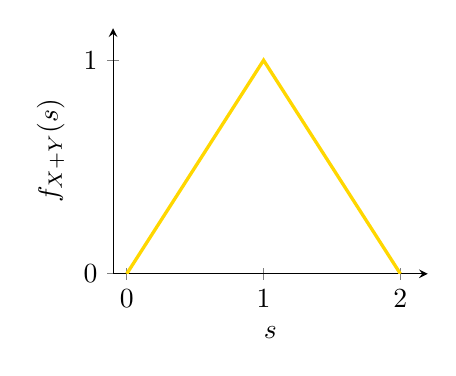
\begin{tikzpicture}\begin{axis}[width=.46\textwidth,height=4.7cm,axis lines=left,xlabel={$s$},ylabel={$f_{X+Y}(s)$},xmin=-.1,xmax=2.2,ymin=0,ymax=1.15,xtick={0,1,2},ytick={0,1}]
\addplot[Gold,very thick]coordinates{(0,0)(1,1)(2,0)};
\end{axis}\end{tikzpicture}
\caption{左：截断后的CDF有跳跃；右：两个独立均匀变量之和的三角密度}\label{fig:mixed-convolution}\end{figure}

\section*{章末分层习题}
\exercise{2-a}{基础}{设$X$在$0,1,2$的概率依次为$c,2c,3c$，求$c$及$F_X(1)$。}
\exercise{2-b}{基础}{$X\sim\Exp(3)$，求$\Pp(1<X\le2)$和中位数。}
\exercise{2-c}{考研风格}{$X\sim U(0,2)$，求$Y=X^2$的CDF与密度。}
\exercise{2-d}{考研风格}{独立$X\sim U(0,1),Y\sim U(0,2)$，求$X+Y$密度。}
\exercise{2-e}{竞赛拓展}{$N\sim\Pois(\lambda)$，求$\Pp(N\text{为偶数})$。}
\exercise{2-f}{竞赛拓展}{独立几何变量$N_1,N_2$成功率均为$p$，求$N_1+N_2$质量函数。}
\exercise{2-g}{测度论选学}{$X\sim U(-2,2)$，$Y=\max(X,0)$，写出$Y$的原子质量和连续部分。}
\exercise{2-h}{测度论选学}{构造仅在$x=0$处改变CDF取值的函数，说明右连续性为何不能忽略。}
\section*{章末方法速查}
\begin{quicktable}
CDF法&任意分布&非单调、原子&端点开闭与漏跳跃\\
逆像密度法&分支可微、连续部分&平方、倒数&漏逆像或雅可比\\
卷积&独立和&寿命和、计数和&积分区间随参数变化\\
生成函数&变换存在且唯一性适用&可加分布族&忽略独立或收敛域\\
\end{quicktable}
